%%==================================================
%% chapter03.tex for BIT Master Thesis
%%==================================================
\chapter{基于地理位置区块链的出租车调度系统框架}
% 基于地理位置区块链的出租车调度系统的目标和研发现状简介。

本章介绍出租车调度系统的框架和流程结构,首先是从整体对系统的架构进行了介绍,然后分别介绍区块链服务端的结构功能,和车辆终端和乘客终端的功能构成,然后对系统的运行流程进行了介绍,包括乘客端的业务流程和车辆端的业务流程设计。
% 本系统采用本章所描述的结构和流程,结合真实地理数据的矢量地图,模拟了真实地理环境,使系统的运行结果更接近真实环境下的运行情况。

\begin{figure}[h]
  \centering
  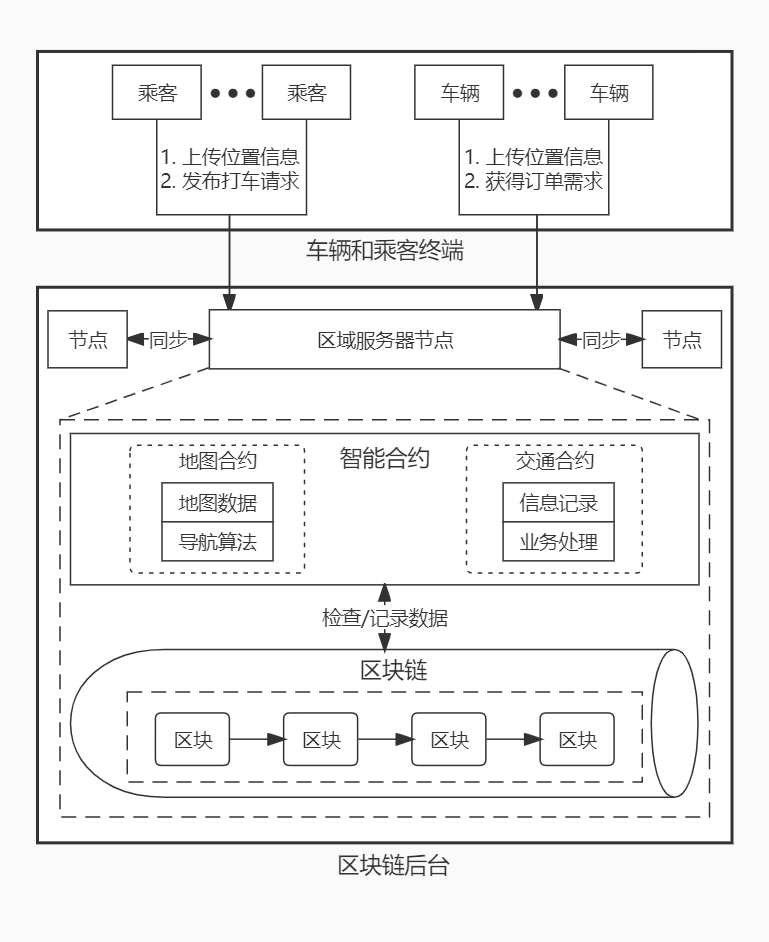
\includegraphics[width=0.9\textwidth]{figures/structure}
  \caption{出租车调度系统架构图}\label{fig:structure}
\end{figure}
% 1. 利用地理位置区块链
% 2. 利用GeoHash的特性
% 3. 优化A*路径规划算法
% 4. 新概念的区域调度
% 5. 实现去中心化的安全的车辆调度系统
% 6. 验证基于GeoHash地理数据和区块链研发自组网应用的可行性

\section{基于地理位置区块链的出租车调度系统架构设计}
% 介绍基于地理位置区块链的出租车调度系统的架构,由区块链后台和浏览器终端构成。
如图\ref{fig:structure}所示。乘客和车辆随身运行的终端与其所属区域内的节点服务器进行交互。区块链后台是指按一定规律分布在城市交通系统中的路边服务节点,其上运行着自动化执行任务的智能合约。因系统后台是基于地理位置区块链的,故其可以通过地理信息相关的功能更好地支持整个系统。乘客和车辆的终端分别执行发单和接单的功能,以此和区块链后台一同构成完整的调度系统。

\subsection{系统的结构说明}
本文出租车调度系统的架构如图\ref{fig:structure},整个系统分为浏览器终端和区块链服务端两大模块,其中浏览器终端分为乘客终端和车辆终端两种。为保证身份信息的匿名性,乘客和车辆的终端之间不会产生直接的信息交互。

乘客终端直接与区块链服务端交互,负责提出打车请求,生成上车点和下车点位置,然后向区块链服务端发送消息,将需求记录在智能合约中。此后,乘客端会保持监听区块链服务端的消息,得到返回的车乘匹配结果。为保证匿名性,乘客端得到的匹配结果中不显示车辆的具体身份信息,但会显示车辆的位置。之后在接客和送客过程中,乘客端会通过监听从区块链服务端获得路径规划的结果。最后,乘客端在被送达目的地之后,会向区块链服务端发送消息,确认自己的订单已完成,具体流程会在3.1.3节描述。

车辆终端直接与区块链服务端交互。车辆终端会周期性向区块链服务端发送消息,维护自己的位置和载客状态。服务端将空载车辆匹配到的乘客上车点位置返回给对应的车辆终端。车辆终端还会根据自己的位置和乘客的起点位置,向区块链服务端请求路径规划并获得结果。在成功接到乘客后,车辆终端会从区块链后台获得乘客的终点位置,然后根据位置向区块链服务端请求路径规划和获得结果。在完成订单后,区块链服务端会将车辆终端置为空载状态,具体流程会在3.1.3节描述。

区块链服务端会接受乘客端和车辆端的发来的位置信息和状态信息并进行记录。在收到乘客终端的打车请求后,会运行智能合约的车乘匹配算法,并将匹配结果双方的位置通知给对应的车辆和乘客。同时,区块链服务端还会根据车辆终端的请求运行路径规划算法,并将结果返回给对应的车辆终端和乘客终端。具体流程会在3.1.2节描述。

\subsection{区块链上智能合约端模块}
% 介绍区块链后台模块的功能。
智能合约运行在地理位置区块链平台上,根据负责的功能不同分为两种合约,第一种是负责记录地理信息和执行路径规划功能的合约,本章中称其为地图合约;第二种是记录乘客和车辆的身份信息和位置信息的合约,本章中称其为交通合约。将智能合约按功能的类型分开,实现了服务端模块之间的解耦,方便了区块链系统的维护,增加了系统的稳定性和可靠性。

地图合约主要由地图存储模块和路径规划算法模块两个模块构成:

(1)地图存储模块:响应乘客和车辆终端根据GeoHash区域发出地图数据查询请求,返回对应区域的矢量地图数据。接收JS脚本上传的GeoHash矢量地图,将地图数据与不同前缀长度的GeoHash区域进行绑定,同时,将地图的三叉及多叉路口连接的道路进行存储,以方便路径规划算法在执行过程中对路口所连接道路的查找。

(2)路径规划算法模块:响应车辆终端的路径规划请求,返回路径规划的结果给对应的车辆和乘客。路径规划算法返回的结果是一个一维数组,其元素是最短路径上所有路段的起止点。路径规划算法模块,是系统进行路径规划的核心部分,其接收的终端请求包括一个起点GeoHash参数和一个终点GeoHash参数,通过支持GeoHash的A*算法进行路径规划运算并返回结果。

除去地图存储和路径规划两个模块外,地图合约还提供了修改算法参数的接口。在以道路长度为权值的路径规划算法中,可以通过接口修改参数从而找到计算性能和准确性最优的参数。除此之外,当交通场景需求发生变化时,需要为导航算法引入不同类型的权值进行路径规划,此接口也可以方便参数的修改,以方便路径规划算法计算不同权值类型下的最短路径结果,拓展了路径规划模块的健壮性。

交通合约主要由信息记录模块和调度处理模块这两个模块组成:

(1)信息记录模块:接收终端发来的包含自己的状态信息和位置信息的消息,初始化和维护车辆和乘客终端的账户信息和位置信息。在初始化时将乘客的乘车状态设置为未乘车,将车辆的载客状态设置为未载客。信息记录模块同时也能改变乘客的乘车状态和车辆的载客状态,方便调度处理模块确定可调度的车辆。完成订单后,信息记录模块还会通知相关车辆乘客的支付状态,方便车辆司机判断是否可以去接下一单需求。此外,信息记录模块还给司机提供了退出系统的功能,即车辆司机需要休息或者遇到特殊情况时,可以适时退出调度系统,避免被分配到未来的需求订单。

(2)调度处理模块:接收乘客的打车请求消息,将乘客和距离乘客最近的空车做匹配,将匹配结果返回给对应的乘客和车辆。乘客提交打车请求后,调度处理模块会根据乘客的位置,遍历乘客所在区域和其周围相邻的区域,寻找距离乘客最近的空车,然后将其分配给乘客。车辆在接到订单并同意后,调度处理模块会将车辆状态改为已载客。总之,调度处理模块主要完成了匹配区域内最近的空车和修改车辆和乘客的乘车状态这两个功能。


\subsection{浏览器终端模块}
% 介绍浏览器终端模块的功能。
乘客终端的功能包括向区块链服务端登录位置信息和账户信息,初始化自己的位置(以GeoHash表示位置),展示乘客自己的位置和周边的矢量地图数据。功能还包括发出乘车请求、确认上车和确认到达终点完成交易。

乘客终端能够从区块链服务端请求到自己位置周边的矢量地图数据。乘客端向区块链服务端发送自己打车的起点和终点位置,然后乘客端可以向区块链服务端发出申请调度车辆的请求,从区块链服务端获得匹配到的车辆位置信息。在完成业务后,乘客通过web3接口发送确认完成交易的消息给区块链服务端,后者将相应车辆的状态改为未载客。

车辆终端的功能包括登录位置信息和账户信息,而且同样具备在前端展示矢量地图数据的功能,可以看到自己的位置信息。如果司机需要休息或者遇到意外情况,终端还提供了退出功能,供车辆退出调度系统,以免接到新的需求订单。同时,车辆终端还具备让司机选择是否接客的功能,在接到乘客订单时,车主可以看到乘客的位置,判断能否顺利接到乘客,如果有困难无法接客可以选择拒绝接受此订单。

车辆终端在进行登录时,直接向区块链服务端模块发送自己的位置信息和账户信息。同时,车辆终端也是直接向区块链服务端申请并获取地图数据。车辆终端模块通过web3接口向区块链服务端申请到乘客上车点的路径规划并获得路径结果。相应的,车辆终端可向区块链服务端申请到乘客目的地的路径规划并获得路径结果。

\section{出租车调度系统流程设计}
% 出租车调度系统的流程设计,出租车接送客业务的企业研究现状,流程介绍。
% 出租车调度系统的流程
首先乘客通过浏览器终端发出乘车请求,将自己的起点和终点传到区块链服务端的智能合约进行记录。智能合约会通过乘客起点的GeoHash获得乘客所在的GeoHash区域,据此进行区域调度(流程如图\ref{fig:region})来寻找最近的空车。通过GeoHash邻居算法找到与乘客起点所在区域相邻的8个区域,加上乘客起点所在的区域共9个区域,在这些区域内寻找合适的车辆,然后将最佳匹配的空车的信息通过web3回调返回给乘客端。

\begin{figure}[h]
  \centering
  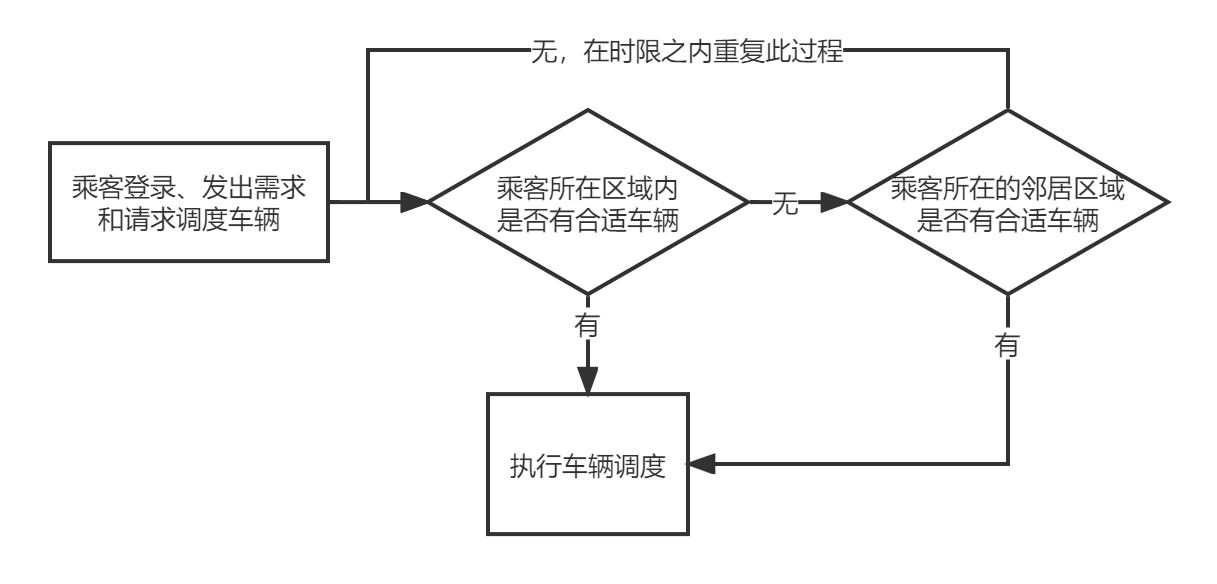
\includegraphics[width=1.0\textwidth]{figures/区域调度车辆流程}
  \caption{区域调度车辆流程}\label{fig:region}
\end{figure}

乘客端在收到车辆信息后,会通知智能合约修改车辆的载客状态和自己的乘车状态。智能合约在接收到请求后会通过assert检查该车辆的载客状态(如图\ref{fig:conflict}),即检查同一车辆是否在短时间内被分配给了不同的乘客。如果状态检查正常,则智能合约认为车辆和乘客匹配成功,顺利修改乘客的乘车状态和车辆的载客状态;如果状态检查不正确,则智能合约认为这次的车辆调度未成功,会通知乘客端重新进行呼车操作,此过程可隐式进行,方便乘客的操作。通过上述流程可以避免同一车辆被同时分配给多个乘客的错误。

\begin{figure}[h]
  \centering
  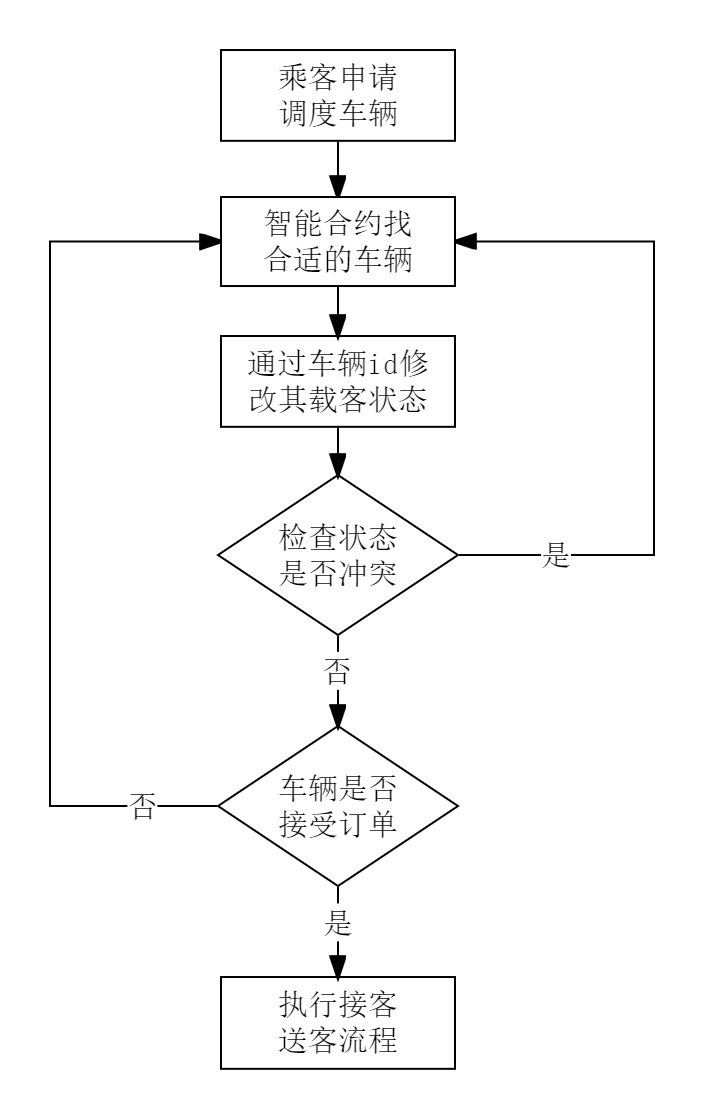
\includegraphics[width=0.6\textwidth]{figures/解决调度冲突}
  \caption{解决调度冲突流程}\label{fig:conflict}
\end{figure}

车辆和乘客匹配成功后,相关的车辆会从智能合约监听到自身的状态变化,即智能合约会把乘客的订单通知到对应的车辆。此时司机可以从终端地图上观察到乘客的位置,同时根据自己的条件和意愿选择是否去接送乘客:如果选择不接送乘客,则会将此选择反馈给智能合约,智能合约会通知乘客订单已经被取消,乘客需重新执行呼车流程,同时智能合约也不会再向原车辆提供乘客相关的信息。

如果车辆确认接送乘客,则如图\ref{fig:routing}所示,服务器端的智能合约会根据车辆位置和乘客的上车点执行路径规划,将路径规划的结果进行存储,并将结果通知给车辆端和乘客端,确保双方获取的路径规划结果一致,车乘双方均可在自己的终端地图观察到路径规划结果。车辆会根据路径规划结果去上车点接到乘客。乘客上车后,车辆确认接到乘客,智能合约会再次执行路径规划算法,通过乘客的上车点和终点得到最优路径,将路径规划结果进行存储,并通知车辆端和乘客端,在双方的地图上显示路径规划结果。车辆会根据最优路径将乘客送到终点。

\begin{figure}[h]
  \centering
  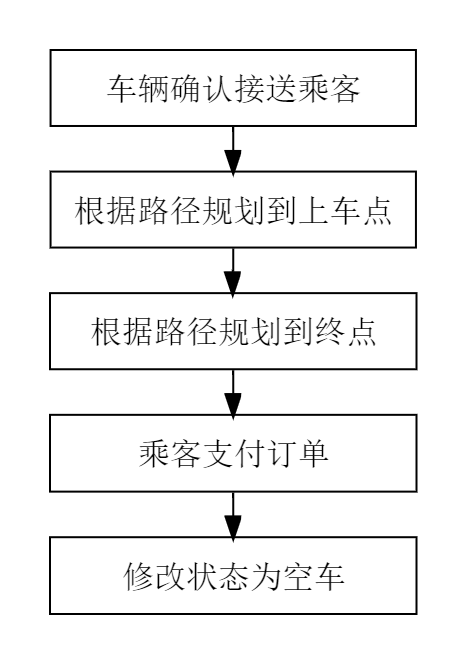
\includegraphics[width=0.4\textwidth]{figures/按导航执行业务}
  \caption{车辆执行业务流程}\label{fig:routing}
\end{figure}

车辆送乘客到达终点后,乘客执行确认到达终点的操作,表示车辆已经按路径规划结果完成任务。智能合约在接收到乘客的确认到达后,会将乘客的状态从已乘车改为未乘车,将车辆的状态从已载客改为未载客,并更新空车的位置,到此完成了一轮完整的业务流程。车辆在收到智能合约的状态改变通知后,可以根据自己当前的地理位置继续等待下一个订单任务。

% \subsection{乘客端业务流程设计}
% 介绍乘客端浏览器的业务流程。
% \subsection{出租车端业务流程设计}
% 介绍出租车端浏览器的业务流程。

\section{系统自动化运行框架的设计}
自动化运行框架基于python语法和selenium库实现,通过自动化操作浏览器运行来模拟车辆终端和乘客终端的行为(如图\ref{fig:auto})。

乘客端的自动化python脚本可以通过设置参数来决定打车乘客的数量。自动化脚本控制每个乘客根据自己的账户信息登录系统,然后按照各自的起止点需求和发布时间来提出打车请求。在智能合约成功记录乘客的起止点需求后,自动化脚本监听到反馈,会控制乘客端开始申请车辆调度。匹配到的车辆在确定接单后,会前来上车点接到乘客,并将乘客送到目的地。自动化脚本监听到乘客到达目的地,会执行确认和支付订单的操作,然后退出浏览器终端,视为乘客完成了一次完整业务。

\begin{figure}[h]
  \centering
  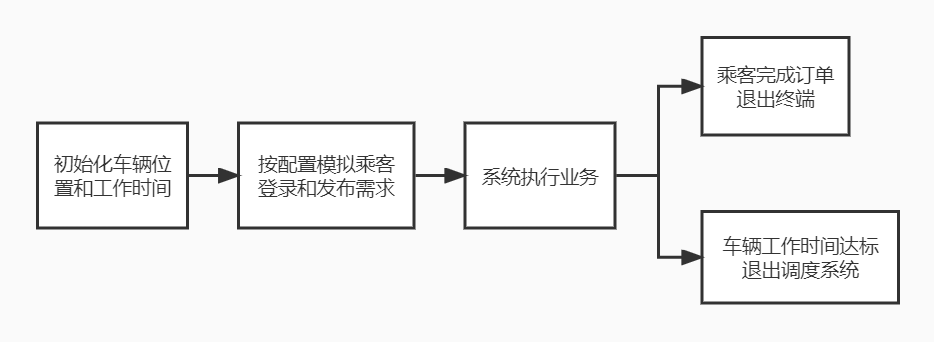
\includegraphics[width=1.0\textwidth]{figures/自动化流程}
  \caption{自动化模拟流程}\label{fig:auto}
\end{figure}

车辆端的自动化脚本控制每辆车根据自己的账户id登录系统并初始化自己车辆的GeoHash位置,在智能合约进行记录。自动初始化完成后,车辆即可通过监听智能合约的通知来获得乘客订单并选择是否确认接受。车辆可根据即时的乘客需求来执行业务流程。此外,自动化脚本可以控制车辆的工作时长,超出工作时长后,相关车辆将会退出系统,智能合约也不再为其提供乘客订单。

\section{本章小结}
本章先在整体上介绍了本文的出租车调度系统结构,然后根据结构图分别描述了车辆端和乘客端的终端功能、区块链后台的结构和功能是如何设计的。接着,本章描述了出租车调度系统的流程设计,系统的流程包括乘客端的发单、付款等业务运行流程和车辆端的确认接单、路径规划等业务运行流程。本文的系统运行实验是基于本章的业务流程,在模拟的网格道路和真实的地图道路上分别进行了实验。